\section{Multi-Layer Perceptron Classifier}\label{sec:MLP}
	    \pagestyle{mario}
	    \sectionauthor{M. Gini \& T. M. Hayden} %\printinunitsof{cm}\prntlen{\linewidth} this shows linewidth in cm

This section presents an MLP classifier designed to classify the CIFAR-10 dataset. The section is organized as follows: Section \ref{subsec:setup} introduces the software setup used to implement the MLP classifier. Section \ref{subsec:preProp} discusses the data preprocessing and augmentation. Section \ref{subsec:netStruct} analyzes the effect of different network structures on performance. Section \ref{subsec:optNet} analyzes the effect of different hyperparameters. Finally, Section \ref{sec:optClassifier} presents the optimized MLP classifier.

\subsection{Software Setup}\label{subsec:setup}

MATLAB's Neural Networks toolbox is employed to implement the MLP classifier. The toolbox provides convenient algorithms and applications to design the MLP. A network training function with a convenient graphical user interface (GUI) to observe the progress is included as well. Figure \ref{fig:NNtool} shows the GUI.

Since this is a classification problem, parts of the network structure are given. The output of the MLP should be a prediction of to which class the input belongs to. This is accomplished with the help of the softmax function, also called normalized exponential function. Equation \ref{eq:softmax} shows the formula of such a function. A softmax layer is then used as the last layer. It gets a $K$-dimensional input vector $\boldsymbol{z}$ of arbitrary real values and "squashes" it into a $K$-dimensional output vector $\sigma(\boldsymbol{z})$ of real values in the range $[0,1]$. In our case, $K=10$ and the output values represent the probabilities that the input belongs to the respective class. The class with the highest probability then constitutes the predicition of the MLP.

\begin{equation}\label{eq:softmax}
\sigma(\boldsymbol{z})_j = \frac{e^{z_j}}{\sum_{k=1}^{K}e^{z_k}}\quad \textrm{for}\quad j = 1,...~K.
\end{equation}

Every ANN will have at the very least one input layer and one output layer. The size of the input layer simply depends on the size of the input data vector. In the case of the CIFAR-10 dataset, the input size is $1\times3072$, the number of pixels per image. Since the dataset is to be classified into 10 categories, the output layer is a softmax layer with 10 nodes.

\begin{figure}[h!]
  	\centering
  	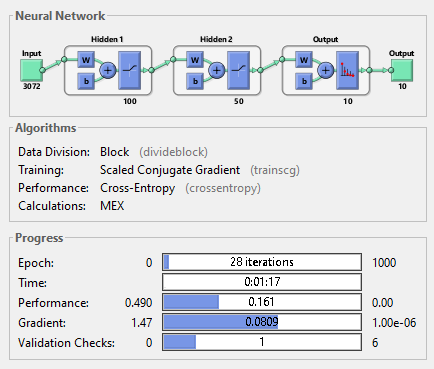
\includegraphics{images/NNtool}
  	\caption{Screenshot of MATLAB's nntraintool.}
  	\label{fig:NNtool}
\end{figure}

The other hidden layers consist of standard MLP. The input to the MLP are the pixel values of the image. Preprocessing and augmentation as described in the next section is done before the pixel values are fed into the network. MATLAB offers lots of adjustable settings for the MLP. Unless mentioned otherwise, the following settings are employed as default settings:

\begin{itemize}
	\item Training function: 'trainscg', the scaled conjugate gradient method.

	\item Loss function: 'crossentropy'

	\item Activation function: 'tansig'

	\item As a default network structure, two hidden layers are employed with 100 and 50 neurons in the first and second layers respectively.

	\item Weight initialization: The weights of the neurons are randomly initialized. Since this leads to slightly different performance for each run, the performance analysis for each configuration is run five times and then the test accuracy is averaged. The standard deviation of the different runs is then plotted as well.

	\item The training batch size is set to 20000 images. This constitutes a compromise between a good performance and a reasonable training time. 80\% are used for training and 20\% are used for validation.

	\item The testing batch consisting of 10000 images is employed for testing of the MLP.
\end{itemize}

\FloatBarrier
\subsection{Data Preprocessing and Augmentation}\label{subsec:preProp}

Data preprocessing and augmentation take place before the data is fed into the network. In the preprocessing step, the data is normalized and centered around the mean. In the augmentation step, the amount of data is augmented through operations like image flipping.

\subsubsection{Data Preprocessing}\label{subsub:dataPreProp}

  	Each image of the dataset is represented by a $32\times32\times3$ array, which results in 1024 pixel values per color channel. To be processed by the MLP, it is first transformed into a $1\times3072$ array. The pixel values are integers in the range [0,255]. For normalization, the data is divided by 255 to lie within the range [0,1]. Accordingly, the datatype changes from the integer type to double. In a second step, the mean per pixel over the whole training set is subtracted. This centers the data per channel.

  	Data preprocessing also includes the division of the complete dataset into appropriate training, validation and test data batches. There are 50000 images available for training. With the default splitting into training and validation dataset (80\% for training and 20\% for validation), Figure \ref{fig:dataPreprocessing} shows the effect of varying the training batch size as well as employing data preprocessing.

  	\begin{figure}
  		\centering
   		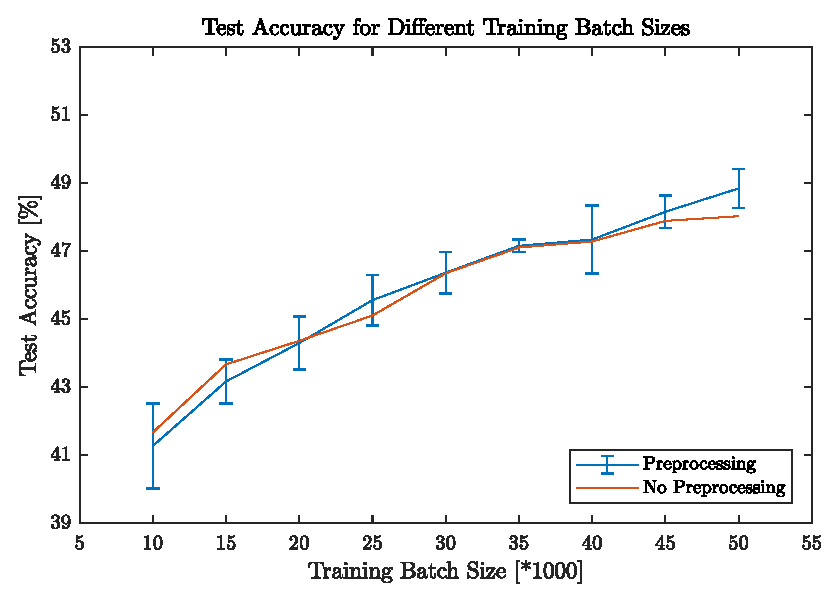
\includegraphics{images/dataPreprocessing}
   		\caption{Comparison of network performance with and without data preprocessing. The errorbars represent one standard deviation. The default MLP classifier is used.}
   		\label{fig:dataPreprocessing}
   	\end{figure}

   	As intuitively expected, the test accuracy increases for an increasing training batch size. However, the data preprocessing does not lead to a significant increase of performance. The normalization and mean subtraction do not have a big influence in the specific case of the CIFAR-10 dataset since the input values already lie in a well defined range and the mean per pixel is also a almost constant value over all pixels.

\subsubsection{Data Augmentation}

Figure \ref{fig:dataPreprocessing} shows that a larger training batch size leads to an increased performance. A natural approach to increase classification accuracy is therefore to increase the training batch size. This can be done artificially by implementing data augmentation. We do this by implementing image flipping and image rotation. Figure \ref{fig:dataAugmentation} illustrates the performance gain by using horizontal mirroring. The test accuracy is significantly increased for all training batch sizes by around \SI{3}{\percent}.

   	\begin{figure}[h!]
		\centering
   	  	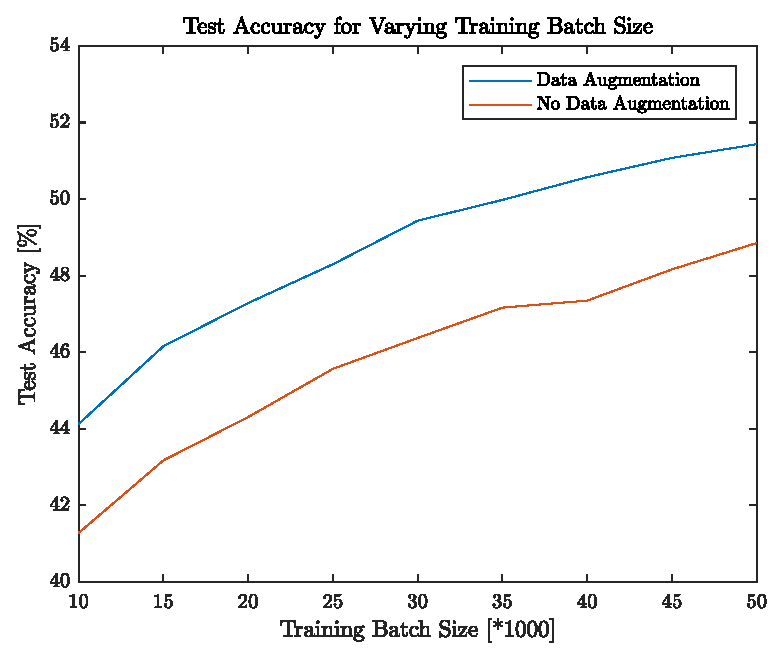
\includegraphics{images/dataAugmentation}
   	  	\caption{Comparison of network performance with and without data augmentation. The errorbars represent one standard deviation.}
   	  	\label{fig:dataAugmentation}
   	\end{figure}

Figure \ref{fig:dataAugDemo} illustrates the data augmentation process on a typical image. The image is mirrored and rotated three times by 90 degrees. This results in a 8-fold increase of the training batch size.

   	\begin{figure}[h!]
   		\centering
   		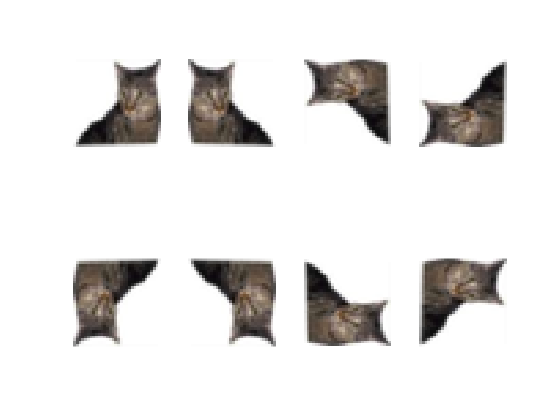
\includegraphics{images/DataAugDemo.png}
   		\caption{Illustration of the data augmentation process on a cat image. Image mirroring and rotation is employed.}
   		\label{fig:dataAugDemo}
   	\end{figure}

\subsection{Optimization of Network Structure}\label{subsec:netStruct}

Choosing the correct architecture of a neural network remains an area of study which is still not fully understood\cite{andersen1999cross}. For a given problem, there is a variety of valid MLP architectures. Approaches to choose an architecture are mostly based on heuristics and therefore not foolproof\cite{andersen1999cross}.

\subsubsection{Number of Hidden Layers}

In general, a MLP can have an arbitrarily large number of hidden layers. However, MLP architectures with a large number of hidden layers are not common. This is because adding more layers increases the chance that the classifier finds a local minimum\cite{de1993backpropagation}. Additional hidden layers rarely result in improved performance. Figure \ref{fig:layers} shows the effect of varying the number of hidden layers of our default MLP classifier. Note that as expected, the test accuracy remains almost constant for more than two hidden layers.

\begin{figure}[h!]
    \centering
    \includegraphics{images/numberlayers}
    \caption{Effect of varying the number of hidden layers of the default MLP classifier. The errorbars represent one standard deviation of the averaging process.}
    \label{fig:layers}
 \end{figure}

\subsubsection{Number of Neurons}

Choosing the optimum number of neurons per layer is a challenging task when designing any MLP architecture. Even in modern archetectures, the number of neurons is generally first estimated using empirical rules and then optimised for the particular dataset\cite{lawrence1998size}. This is especially the case when using noisy datasets such as CIFAR-10.

Figure \ref{fig:surfaceLayers} shows the result of varying the number of neurons using two hidden layers with our default MLP. The results show that the number of neurons in the first layer have very little effect on the test accuracy. In addition, the results also show that increasing the number of neurons beyond around 70 had very little to no effect. Increasing the number of neurons also increased the time to train. The number of neurons in the second layer also has a much stronger impact on the time taken to train than the number of neurons in the first layer.

	\begin{figure}[h!]
   		 \centering
   		 \includegraphics{images/surfacelayers}
   		 \caption{Surface plot showing the effect of varying the number of neurons in the hidden layers of the MLP}
   		 \label{fig:surfaceLayers}
    \end{figure}

\subsection{Optimization of Network Hyperparameters}\label{subsec:optNet}

Hyperparameter selection for ANN such as MLP has become an active field of research with various algorithms being used to estimate optimal parameters\cite{bergstra2011algorithms}. However, since these algorithms rely on performing many trials and updating the parameters accordingly, they proved unsuitable for our purposes due limited computational resources. Instead, a few parameter are varied whilst using the default MLP structure. Optimal parameters are then estimated from the observed trends.
%\subsubsection{Learning Rate}
%
%Choosing the learning rate for a MLP classifier can be a challenging process. There is no approach that will work optimally for every dataset. A learning rate that is too high can overshoot the solution and become unstable. However low learning rates can become stuck in local minima or take a long time to train. A good solution is to pick a high learning rate that can pass over local minima and  to gradually decrease the learning rate so that the classifier does not become unstable. This will result in a classifier which initially follows general trends and 'explores' a large portion of the parameter space. Later on the smaller learning rate will allow for the model to be fine tuned into a particular solution.
%
%The effects of changing the learning rate in our model can be seen in Figure \ref{fig:learningRate}. The figure shows that increased learning rates, in general, had a positive effect on model accuracy.
%
%\begin{figure}[h!]
%    \centering
%    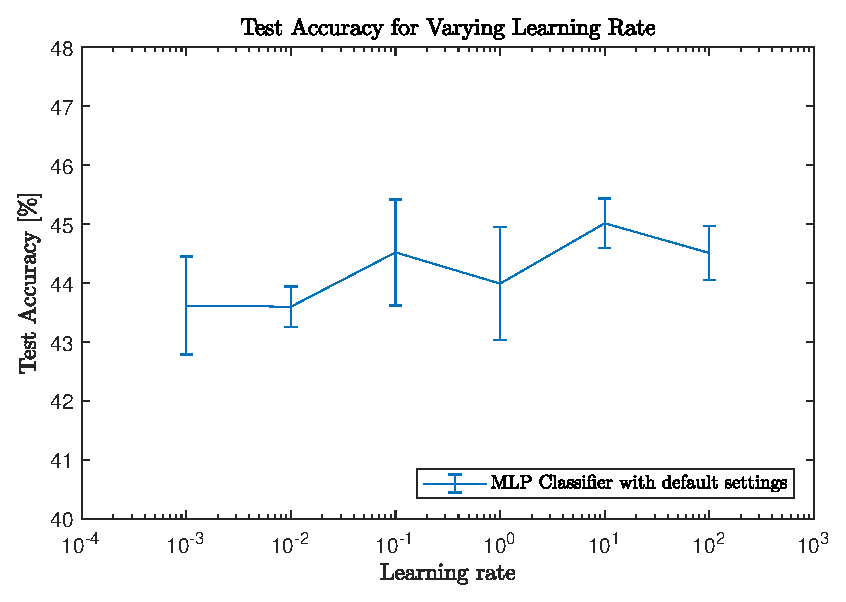
\includegraphics{images/learningRate.eps}
%    \caption{Comparison of the test accuracy of the default MLP using different learning rates.}
%    \label{fig:learningRate}
% \end{figure}
%\FloatBarrier

 \subsubsection{Performance Function}

 The performance function is used to measure the error that a specific input produces in the network. The error expression is then used in the training algorithm to update the weights of the model\cite{hecht1988theory}. MATLAB offers the following different performance functions:

 \begin{itemize}
 	\item SAE, the sum absolute error function
 	\item SSE, the sum squared error function
 	\item MAE, the mean absolute error function
 	\item MSE, the mean squared error function
 	\item Cross-entropy error function
 \end{itemize}

 Figure \ref{fig:performFct} shows that three performance functions result in a similar performance: MSE, SSE and Cross-entropy. SAE and MAE result in a slightly lower performance. An explanation might be that these two functions take the absolute error instead of the squared error. Using the squared error leads to a stronger penalization of larger errors. The best performance is achieved using the cross-entropy performance function. This performance function heavily penalizes large errors with very little penalty for small errors. It is also recommended by MATLAB for classification tasks.

 \begin{figure}[h!]
 	\centering
 	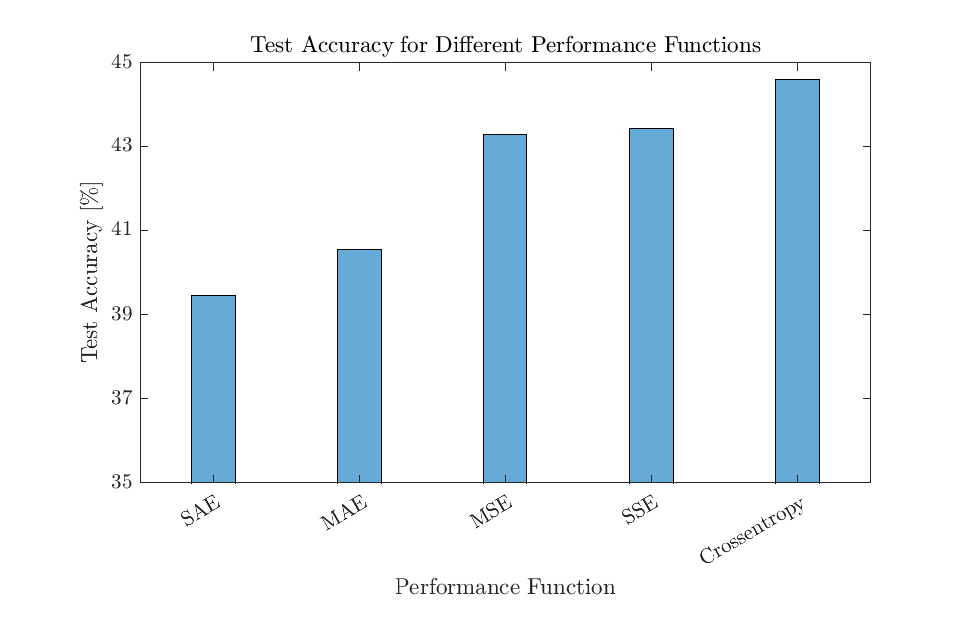
\includegraphics{images/performFct}
 	\caption{Comparison of the test accuracy of the default MLP using different performance functions.}
 	\label{fig:performFct}
 \end{figure}

 \subsubsection{Activation Function}

 The activation function controls the firing of a single neuron. After multiplying the input with the weight and bias vector, the result is fed into the activation function. The output of the activation function constitutes the output of the neuron. Again, MATLAB offers a variety of different activation functions. For the sake of completeness, all activation functions are tested with the default MLP. The result is displayed in Figure \ref{fig:activationFct}.

 \begin{figure}[h!]
 	\centering
 	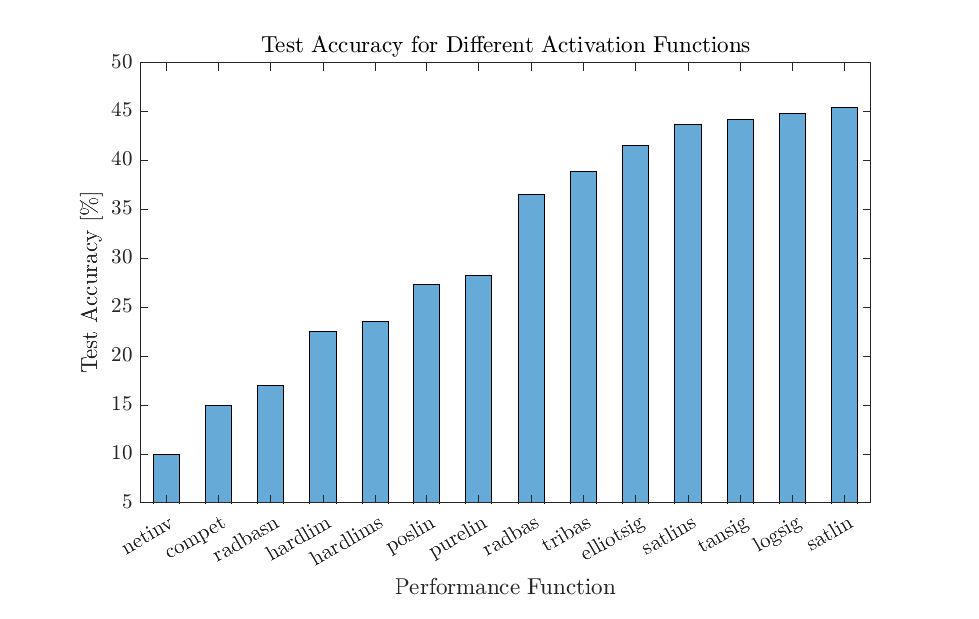
\includegraphics{images/activationFct}
 	\caption{Comparison of the test accuracy of the default MLP using different activation functions.}
 	\label{fig:activationFct}
 \end{figure}

 It can be seen that several activation functions are not suited for a MLP classification problem, e.g the 'netinv' and 'compnet' type. Furthermore, there is a class of activation functions which are very similar and all perform well on that specific problem. Specifically, sigmoid shaped activation functions seem to be the appropriate choice for our problem setting. 'tansig' and 'logsig' are quite similar and 'satlin' and 'satlins' can be viewed as linear approximations of those nonlinear activation functions. It is interesting to note that using the 'satlin' type results in the best performance.

\subsubsection{Training Function}

 The training function is the algorithm that dictates the training process of the network. Once again, MATLAB offers a wide selection of training algorithms. Most are variations of the backpropagation algorithm. Figure \ref{fig:trainingFct} shows the results of using various training algorithms on the default MLP structure.

 \begin{figure}[h!]
 	\centering
 	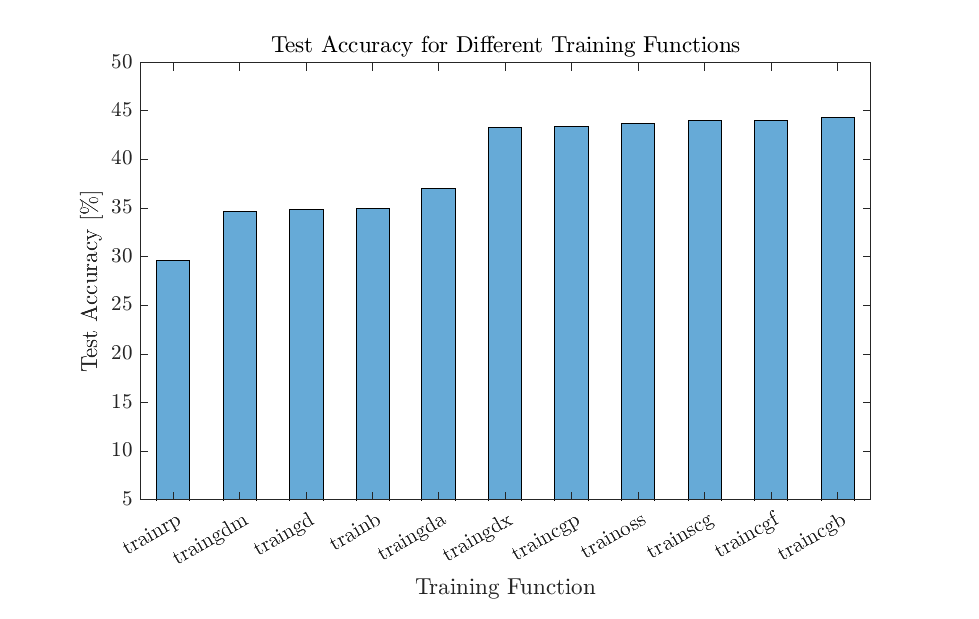
\includegraphics{images/trainingFct}
 	\caption{Comparison of the test accuracy of the default MLP using different training functions.}
 	\label{fig:trainingFct}
 \end{figure}

 All variations of the conjugate gradient backpropagation algorithm\cite{moller1993scaled} achieve good performance. It is interesting that the performance is superior compared to variations of simple gradient backpropagation. 'traindx' which uses momentum is the only gradient backpropagation variation which achieves similar performance than conjugate gradient backpropagation.

 An advantage of conjugate gradient backpropagation algorithms is that they do not require a learning rate parameter. Since our investigations show that they are superior over other backpropagation methods, no further analysis on finding optimal learning rates is conducted.

\subsection{Optimized Classifier}\label{sec:optClassifier}

We now attempt to use the information we have gathered to create our final MLP classifier. The parameters used are summarised below.
\begin{itemize}
    \item Training batch size is set to all 50000 images. This will give the classifier the most data to work with and has consistently given the best results.
    \item Horizontal mirroring is used to augment the data.
    \item Data is mean normalised between $-0.5$ and $0.5$. This has been shown to improve results slightly.
    \item The scaled conjugate gradient backpropagation training function is used. This algorithm proved to be quite fast and gives good results.
    \item The architecture will use two hidden layers with a softmax final layer. Both hidden layers have 100 neurons. Testing on the whole data set revealed that an increased number of neurons in the first layer improved results slightly.
    \item The cross-entropy performance function is used as this gives the highest performance.
    \item The saturating linear activation function is used as this gives the highest performance.
\end{itemize}

Using these results we managed to get a result of $52.61\%$. The confusion matrix is shown in figure \ref{fig:Conf_Matrix}. Table \ref{Tab:Classes} shows how the labels used in the model correspond to real class categories. Note that the highest misclassification exhibited in the confusion matrix is between cats and dogs. This is not surprising as the general form of cats and dogs are quite similar and the poses of both vary considerably throughout the data set.

The MLP was most effective at classifying the ship class. This is because the ship class generally has many distinctive features such as a blue background. In contrast, the dog class performed the worst. The dogs can appear with a variety of colours, poses, backgrounds and scene prominence. This makes it a challenging category to classify.

The MLP took 35 minutes to train and is capable of classifying the entire test set in under 1 second.



\begin{figure}[h!]
   \centering
   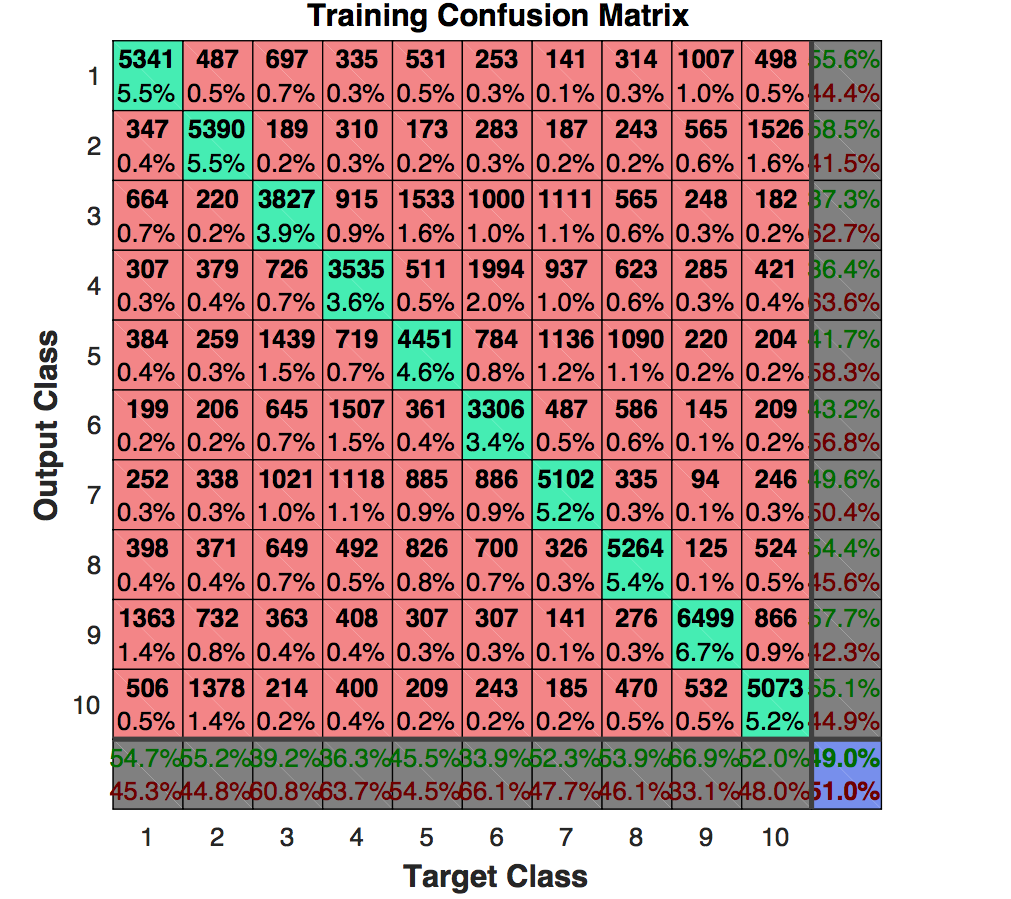
\includegraphics[width=\textwidth]{images/Confusion_Matrix}
   \caption{Confusion Matrix for the final MLP classifier }
   \label{fig:Conf_Matrix}

\end{figure}

\begin{table}[h]
\begin{center}
 \begin{tabular}{||c | c||}
 \hline
 \textbf{Label} & \textbf{Class} \\ [0.5ex]
 \hline
 1& Airplane\\
 2& Automobile \\
 3& Bird\\
 4& Cat\\
 5& Deer\\
 6& Dog\\
 7& Frog\\
 8& Horse\\
 9& Ship\\
 10& Truck\\[1ex]
 \hline

\end{tabular}
\caption{The different classes in the CIFAR-10 dataset.}
\label{Tab:Classes}
\end{center}
\end{table}

\subsubsection{Possible improvements}

There are many improvements which could improve the accuracy of our MLP classifier. Perhaps the simplest and most effective of these is to use more data augmentation. For our final model we only used horizontal mirroring due to RAM constraints. Image rotations and translations are both commonly used to increase performance in image recognition neural networks. In addition, other advanced data augmentation methods, such those used in the fractional max-pooling architecture\cite{graham2014fractional}, could be used.

With more computational power and RAM, it would be possible to do a more thorough hyperparameter search. In particular the number of neurons used in the hidden layers is likely not optimal. A more thorough approach would be to test different numbers of neurons on the entire augmented dataset.

Weight initialization should also be investigated. For our MLP, we simply used a random initialization. However as discussed in section \ref{sec:LSUV}, a good initialization was shown to improve preference of a CNN. It is likely that a similar method could also improve results for an MLP.

In addition, it may be possible to improve the validation process. Our model uses a hold out validation strategy. This involves reserving a section of the data to be used as the validate. There are alternative approaches such as k-fold cross validation which have been shown to produce better results\cite{blum1999beating}.

\FloatBarrier
